\documentclass[10pt, a4paper]{article}
\usepackage[utf8]{inputenc}
\usepackage{pdflscape}
\usepackage{amssymb}
% \usepackage[margin=3cm]{geometry}
\usepackage{graphicx}
\usepackage{oz}
\usepackage{array,multirow,makecell}
\setcellgapes{1pt}
\usepackage[top=4cm,bottom=4cm,left=3cm,right=3cm]{geometry} %marges
\newcolumntype{R}[1]{>{\raggedleft\arraybackslash }b{#1}}
\newcolumntype{L}[1]{>{\raggedright\arraybackslash }b{#1}}
\newcolumntype{C}[1]{>{\centering\arraybackslash }b{#1}}

\title{Analyse Projet BDD}
\date{}
\begin{document}


\maketitle
\tableofcontents
\newpage

\section{Analyse du problème}
\subsection{Hypothèses}
Pour la conception, nous avons fait les choix suivants:
\begin{enumerate}
    \item Le statut des commandes n'est pas dans l'entité mère COMMANDES 
mais dans ses sous-entités afin d'éviter d'avoir des statuts non cohérents 
pour un type de commande donné.
    \item Nous avons rajouté le statut ``terminée'' qui indique qu'une 
commande a effectivement été effectuée et que l'on peut donner un 
évaluation
    \item % TODO: Rajouter le fait qu'on décide de ne pas créer un nouvel identifiant lorsqu'on fait appel au droit a l'oubli
    \item % TODO: Les restaurants s'occupent d'actualiser les statuts de la base de données
\end{enumerate}

Nous sommes arrivés avec les contraintes suivantes :
\begin{landscape}
\subsection{Contraintes}

\begin{center}
\[
\begin{tabular}{|C{5cm}|C{5cm}|C{5cm}|C{5cm} |}

\hline
DF& C. Valeurs 
& C. Contextuelles & C. Multiplicité\\
\hline

RMail $\rightarrow$ RNom, RNumero, RAdresse, Places, 
Presentation, RNote & RType $\in$ \{livraison, emporter, place\} & $\sum 
\mbox{nbPers}  \le \mbox{Places} $ pour un restaurant et ses commandes 
associées & RMail $\twoheadrightarrow$ JourPlage\\

 & Places $> 0$ & $\mbox{Ext(CEId)} \cap \mbox{Ext(CPId)} \cap 
\mbox{Ext(CLId)} = \emptyset $ &  RMail  $\twoheadrightarrow$ 
TypeCommande\\ 
 
 & RNote $\in  [0,5] $ &  $\mbox{Ext(CEId)} \cup \mbox{Ext(CPId)} \cup 
\mbox{Ext(CLId)} = \mbox{Ext(CId)}$ & RMail $\twoheadrightarrow$ PId\\
\cline{1-2}

(PId, Restaurant) $\rightarrow$ PNom, PDescription, PPrix & PPrix $>0$ & 
CPArrivee $\in$ JourPlage pour un restaurant et ses commandes associées & 
RMail $\twoheadrightarrow$ CatNom\\
\cline{1-2}

U\_Id $\rightarrow$ UMail, UMdp, UNom, UPrenom, UAdresse && CDate donne JourPlage pour toute commande& (PId, RMail) $\psur$ ANom \\
\cline{1-2}

CId $\rightarrow$ CDate, CPrix & CPrix $>0$ & CDate $\le$ EDate& 
CId $\twoheadrightarrow$ (PId, RMail)\\
\cline{1-2}

CLId $\rightarrow$ CLAdresse, Indications, CLArrivee, CLStatut & 
CLStatut $\in$ \{ attente, validée, en livraison, annuleeC, annuleeR, 
terminee \}&
EId $\Rightarrow$ CId.statut = \{terminee\}
& CId $\rightarrow$ TypeCommande \\ 
\cline{1-2}

CEId $\rightarrow$ CEStatut &
CEStatut $\in$ \{ attente, validée, disponible, annuleeC, annuleeR, terminee \}&  & CId $\rightarrow$ U\_Id\\
\cline{1-2}

CPId $\rightarrow$ NbPers, CPArrivee, CPStatut &
CPStatut $\in$ \{ attente, validée, annuleeC, annuleeR, 
terminee \}&  & CId $\pfun$ 
EId\\

& NbPers $>0$ & & CatNom $\pfun$ CatNom\\
\cline{1-2}

EId $ \rightarrow$ EDate, Avis, ENote & ENote $ \in [0..5] $&
CType $\in$ TypeCommande pour un CId donné et le RMail associé &\\ 
\cline{1-2}

& JourHeure $\in $ \{LM, LS, MM, MS, MeM, MeS, JM, JS, VM, VS, SM, SS, DM, 
DS \} & & \\
\hline

\end{tabular}
\]
\end{center}


\newpage
\subsection{Diagramme Entités/Associations}
On obtient ensuite le diagramme Entité-Relation suivant:
\begin{center}
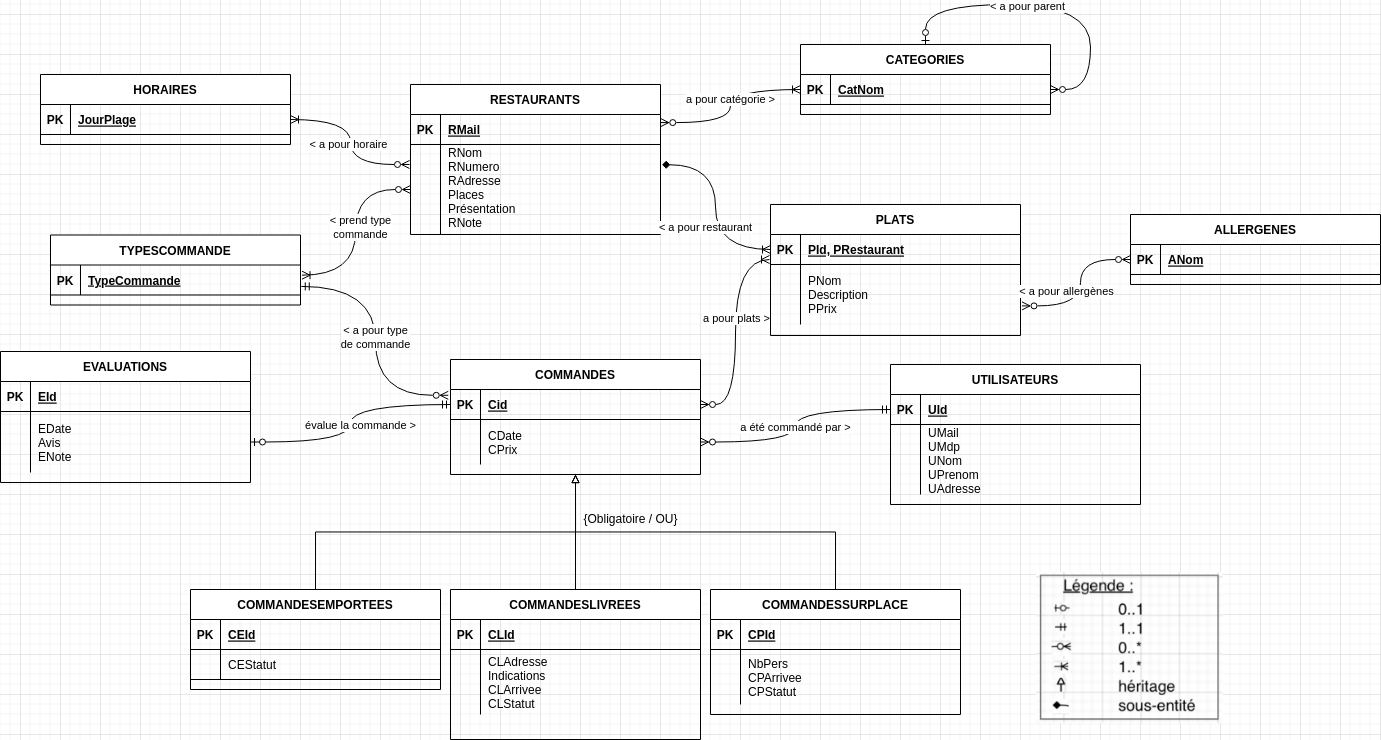
\includegraphics[scale=0.7]{Diagramme_entite_relation.png}\\
\end{center}

\end{landscape}
\section{Modèle Relationnel}


Nous avons appliqué l'algorithme vu en cours pour obtenir le schéma relationnel.

\subsection{Traduction des entités simples}

Nous avons identifié les entités simples suivantes:

\begin{itemize}
    \item Restaurant\@(\underline{RMail}, RNom, RNum, RAdresse, Places, Présentation, RNote)
    \item Commandes\@(\underline{Cid}, CDate, CPrix, \textbf{Uid}, \textbf{TypeCommande})
    \item Utilisateurs\@(\underline{U\_id}, UMail, UMdp, UNom, UPrenom, UAdresse)
    \item Evaluation\@(\underline{Eid}, EDate, Avis, ENote, \textbf{Cid})
    \item Horaires\@(\underline{JourPlage})
    \item TypesCommande\@(\underline{TypeCommande})
    \item Categories\@(\underline{CatNom})
    \item Allergenes\@(\underline{ANom})
\end{itemize}

\subsection{Sous-types d'entités}

Pour une question d'espace occupé nous avons décidé de traduire l'héritage des différentes catégories des commandes par référence. 
Contrairement à l'unification cela nous permet de ne pas avoir à gérer les contraintes avec l'application.

\begin{itemize}
    \item CommandesEmportees\@(\underline{CEid}, CEStatut)
    \item CommandesLivrees\@(\underline{CLid}, CLAdresse, Indications, CLArrivee, CLStatut)
    \item CommandesSurPlace\@(\underline{CPid}, NbPers, CPArrivee, CPStatut)
\end{itemize}

\subsection{Type d'entité faible}

\begin{itemize}
    \item Plats\@(Pid, PRestaurant, PNom, Description, PPrix)
\end{itemize}

\textbf{Contrainte induite par la traduction}: Vérifier que tout restaurant a au moins un plat 

\subsection{Types d'associations}

\subsubsection{Cardinalité 1..1}



\subsubsection{Cardinalité 0..1}



\subsubsection{Cardinalité ?..*}

\section{Analyse des fonctionnalités}
\section{Bilan du projet}
\section{Mode d'emploi}



\end{document}


